\documentclass{article}
\usepackage{fullpage}
\usepackage{dot2texi}
\usepackage{tikz}                                                                                               
\usetikzlibrary{shapes,arrows}  

\usepackage{syntax,multicol}

\author{TJ Ellis}
\title{ECE 683 Compiler Theory\\Final Project}

\newenvironment{grammar*}{\bfseries\begin{grammar}}{\end{grammar}\rmfamily}

\begin{document}
\maketitle
% \section{Scanner}

% \begin{figure}[h]
% \centering
% 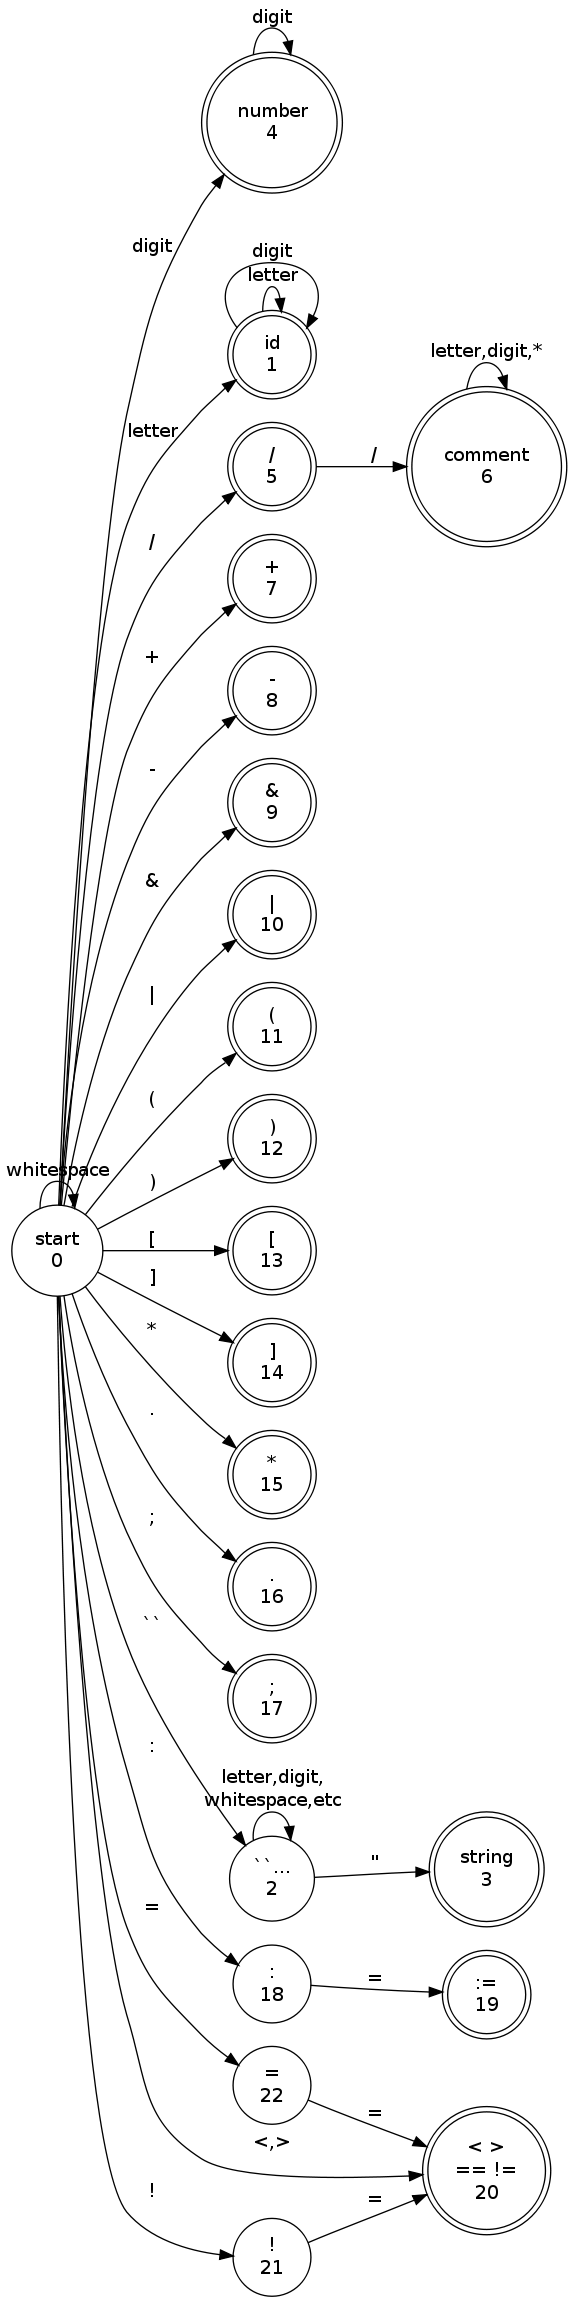
\includegraphics[height=\textheight]{scanner.png}
% \caption{Scanner State Machine}
% \end{figure}

% \subsection*{Keywords}
% \begin{multicols}{2}
% \begin{itemize}
% \item function
% \item begin
% \item end
% \item integer
% \item boolean
% \item string
% \item if
% \item then
% \item else
% \item while
% \item case
% \item is
% \item when
% \item default
% \item and
% \item or
% \item not
% \end{itemize}
% \end{multicols}

\section{Parser}
\subsection{Left Factored Grammar with Left Recursion Eliminated}
The original grammar provided had a few ambiguous production choices
that needed to be left-factored and a few left-recursive rules that
needed to be eliminated. Specifically, \synt{function_call} and
\synt{name} both started with \synt{identifier} and needed to be left
factored, and \synt{expression}, \synt{arithOp}, and \synt{relation}
are left recursive in the original grammar. Below is the updated
grammar, left factored and with left recursion eliminated. ($\lambda$
is the empty string.)

\begin{grammar*}
  <function_declaration> ::= <function_header> <function_body>

  <function_header> :: = 
  function\\
  <identifier>  ( [<parameter_list>] )

  <parameter_list> ::=\\ 
  <parameter> , <parameter_list>
  \alt <parameter>

  <parameter> ::= <type_mark> <variable_declaration>

  <function_body> ::= 
  ( <declaration>  ; )*\\
  begin\\
  ( <statement> ; )*\\
  end function

  % <declaration> ::=
  % <function_declaration>
  % \alt <variable_declaration>

  <declaration> ::=
  <type_mark> <declaration2>

  <declaration2> ::=
  <function_declaration>\alt <variable_declaration>

  <variable_declaration> ::= <identifier> [ [ <array_size> ] ]

  <type_mark> ::=
  integer
  \alt boolean
  \alt string

  <array_size> ::= <number>

  <statement> ::=\\
  <assignment_statement>
  \alt <if_statement>
  \alt <while_statement>
  \alt <case_statement>

%  <function_call> ::=\\
 % <identifier> ( [<argument_list>] )

  <assignment_statement> ::=\\
  <destination> := <expression>
  
  <destination> ::= 
  <identifier> [ [ <expression> ] ]

  <if_statement> ::=
  if <expression> then ( <statement> ; )+\\\ 
  [ else ( <statement> ; )+ ]\\
  end if

  <while_statement> ::=
  while <expression> ( <statement> ; )*\\
  end while

  <case_statement> ::=
  case <expression> is\\
  (when <number> then ( <statement> ;)+)+\\\ 
  [ default then ( <statement> ; )+ ]\\
  end case

  <identifier> ::= [a-zA-Z][a-zA-Z0-9_]*

  % <expression> ::=
  % <expression> and <arithOp>
  % \alt <expression> or <arithOp>
  % \alt [ not ] <arithOp>

  <expression> ::= [ not ] <arithOp> <expression2>

  <expression2> ::=  and <arithOp> <expression2>
  \alt or <arithOp> <expression2>
  \alt $\lambda$

  <arithOp> ::= <relation> <arithOp2>

  <arithOp2> ::= + <relation> <arithOp2>
  \alt - <relation> <arithOp2>
  \alt \& <relation> <arithOp2>
  \alt | <relation> <arithOp2>
  \alt $\lambda$

  <relation> ::= <term> <relation2>
  
  <relation2> ::= \textless  $\;\;$<term> <relation2>
  \alt \textgreater $\;$<term> <relation2>
  \alt == <term> <relation2>
  \alt != <term> <relation2>
  \alt $\lambda$

  <term> ::= 
  <factor> * <term>
  \alt <factor> / <term>
  \alt <factor>

  <factor> ::=  
  ( <expression> )
  \alt  <function_call>
  \alt <name> 
  \alt <number> 
  \alt <string>

  <starts_with_ID> ::= <identifier> <name_or_function_call>
  
  <name_or_function_call> ::= [ [ <expression> ] ] \alt ([argument_list])

  <argument_list> ::=
  <expression> , <argument_list>
  \alt <expression>

  <number> ::= [0-9]+

  <string> :: = “[a-zA-Z0-9_ ]*”
\end{grammar*}

% \section{Syntactic Analysis}
% \section{Code Generation}
% \section{Runtime System}

\end{document}
